\documentclass{standalone}

\usepackage{../thesis}

\usepackage{tikz} 
\usepackage{pgfplots} % drawing plots right here in this file!
\pgfplotsset{compat=1.9} % latest stable release

\begin{document}
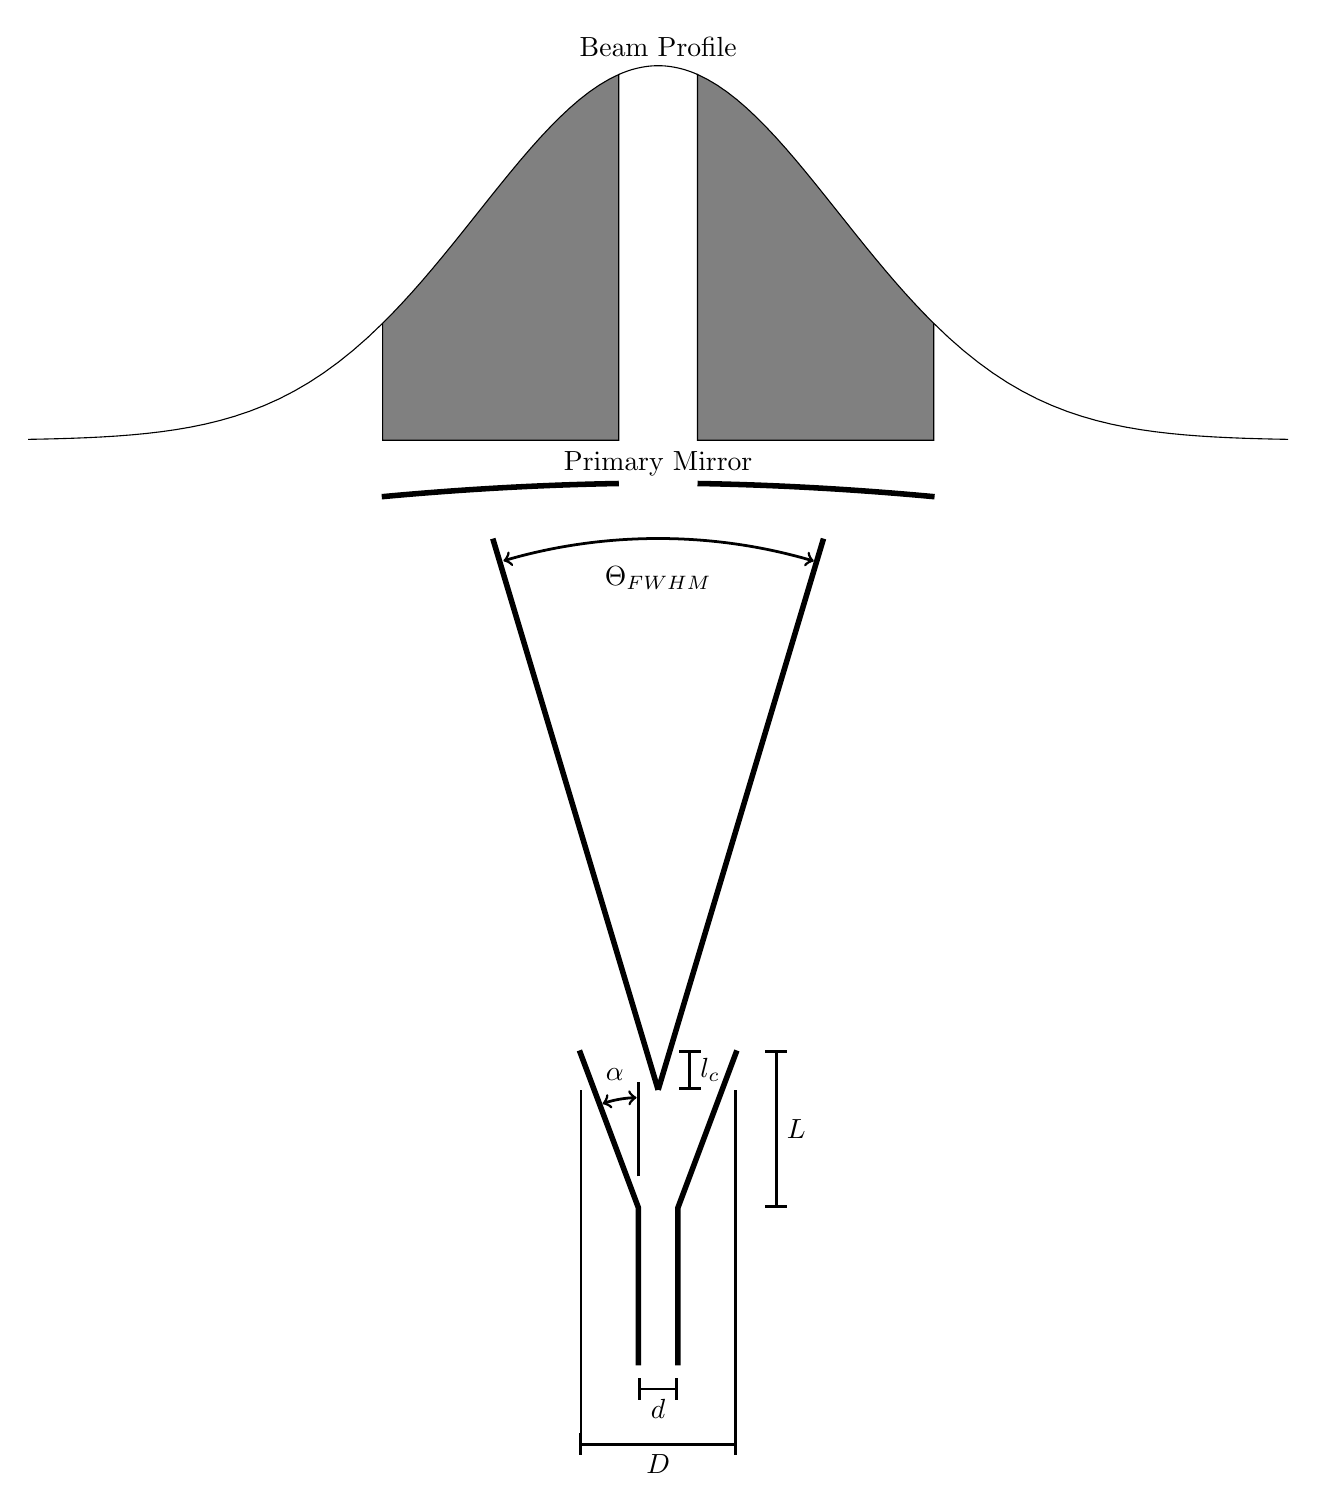
\begin{tikzpicture}
	
	\pgfmathsetmacro{\d}{0.5}
	\pgfmathsetmacro{\l}{2.0}
	\pgfmathsetmacro{\D}{2}
	\pgfmathsetmacro{\L}{2}
	\pgfmathsetmacro{\phcy}{\l + \L - 0.5}
	\pgfmathsetmacro{\phcy}{\l + \L - 0.5}


	% pgf functions
	\pgfmathdeclarefunction{gauss}{2}{%
	\pgfmathparse{1/(#2*sqrt(2*pi))*exp(-((x-#1)^2)/(2*#2^2))}}
	
	% draw feedhorn and dimensions
	\draw[line width=2] (-\d/2,0) -- ++(0,\l) -- (-\D/2,\l + \L);
	\draw[line width=2] (\d/2,0) -- ++(0,\l) -- (\D/2,\l + \L);
	\draw[line width=1,|-|] (-\d/2,-0.3) -- +(\d,0) node[midway,below] {$d$};
	\draw[line width=1,|-|] (\D/2+0.5,\l) -- +(0,\L) node [midway,right] {$L$};
	\draw[line width=1,|-|] (\D/2-0.6,\phcy) -- (\D/2-0.6,\l+\L) node [midway,right] {$l_c$};
	\draw[line width=1,|-|] (-\D/2,-1) -- +(\D,0) node[midway,below] {$D$};
	\draw[line width=1] (-\D/2+0.02,-1) -- +(0,1 + \l + \L - 0.5);
	\draw[line width=1] (\D/2-0.02,-1) -- +(0,1 + \l + \L - 0.5);
	

	\draw[line width=1] (-\d/2,\l + 0.4) -- +(0,1.2);
	\draw[line width=1,<->] (-\d/2,\l) ++ (91:1.4) arc (91:109:1.4);
	\node at (-\d/2 - 0.3,\l + 1.7) {$\alpha$};
	
	% draw beam and dimension
	\draw[line width=2] (0,\phcy) -- +(-0.3*7,7) ;
	\draw[line width=2] (0,\phcy) -- +(0.3*7,7) ;
	\draw[line width=1,<->] (0,\phcy) ++(73.6:7) arc (73.6:106.3:7);
	\node at (0,\phcy+6.5) {$\Theta_{FWHM}$};
	
	% draw beam
	\begin{axis}[axis lines=none,anchor=origin, at={(0,11.75cm)},x=1cm]
		\addplot[domain=-8:-3.5] {gauss(0,(12.5-\phcy)*2*0.3/2.35482)};
		\addplot[domain=-3.5:-0.5,fill=gray] {gauss(0,(12.5-\phcy)*2*0.3/2.35482)} \closedcycle;
		\addplot[domain=-0.5:0.5] {gauss(0,(12.5-\phcy)*2*0.3/2.35482)};
		\addplot[domain=0.5:3.5,fill=gray] {gauss(0,(12.5-\phcy)*2*0.3/2.35482)} \closedcycle;
		\addplot[domain=3.5:8] {gauss(0,(12.5-\phcy)*2*0.3/2.35482)};
	\end{axis}
	\node at (0,16.75) {Beam Profile};
	
	% draw primary mirror
	\draw[line width=2] (-0.5,11.2) arc (91:91 + 4.32:40);
	\draw[line width=2] (0.5,11.2) arc (89:89 - 4.32:40);
%	\draw[line width=2] (0,11.2) arc (90:85:40);
	\node at (0,11.45) {Primary Mirror};
	
\end{tikzpicture}
\end{document}
